\documentclass[letterpaper,12pt]{article}
\usepackage[spanish]{babel}
\usepackage[utf8]{inputenc}
\usepackage{graphicx}
\usepackage{geometry}
\usepackage{titlesec}
\usepackage{fancyhdr}
\usepackage{tcolorbox}
\usepackage{array}
\usepackage{tabularx}
\usepackage{hyperref}
\usepackage{float}
\usepackage{enumitem}
\usepackage{listings}
\usepackage{xcolor}

% ==================== CONFIGURACIÓN DE PÁGINA ====================
\geometry{top=3.5cm, bottom=3cm, left=2.5cm, right=2.5cm, headheight=2cm, footskip=2cm}

% ==================== FORMATO DE TÍTULOS ====================
\titleformat{\section}{\large\bfseries}{\thesection.}{0.6em}{}
\titleformat{\subsection}{\normalsize\bfseries}{\thesubsection}{0.6em}{}

% ==================== ENCABEZADO Y PIE ====================
\pagestyle{fancy}
\fancyhf{}
\fancyfoot[C]{\thepage}
\renewcommand{\headrulewidth}{0.4pt}
\rhead{\textit{Tarea ELO323 / IPD438}}
\lhead{\textit{Emulando Redes con GNS3}}

% ==================== HIPERVÍNCULOS ====================
\hypersetup{
    colorlinks=true,
    linkcolor=blue,
    urlcolor=blue,
    citecolor=blue
}

% ==================== ESTILO PARA CÓDIGO / COMANDOS ====================
\definecolor{codegray}{gray}{0.95}
\lstset{
    basicstyle=\ttfamily\small,
    backgroundcolor=\color{codegray},
    frame=single,
    breaklines=true,
    columns=fullflexible,
    keepspaces=true,
    xleftmargin=0.5cm,
    xrightmargin=0.5cm,
    aboveskip=8pt,
    belowskip=8pt
}

% ==================== CAJA PARA NOTAS ====================
\newtcolorbox{nota}{colback=yellow!8!white, colframe=orange!70!black, title=Nota, fonttitle=\bfseries}

% ==================== MACRO PARA PLACEHOLDER DE FIGURAS ====================
% Uso: \figplaceholder{descripcion del contenido}{texto del caption}
% Reemplace por \includegraphics cuando tenga las capturas.
\newcommand{\figplaceholder}[2]{%
    \begin{figure}[H]
        \centering
        \fbox{\begin{minipage}[c][4.5cm][c]{0.8\textwidth}
            \centering \textit{[ Espacio reservado para captura ]}\\[0.3cm]
            \small #1
        \end{minipage}}
        \caption{#2}
    \end{figure}%
}

\begin{document}

% ==================== PORTADA ====================
\thispagestyle{empty}

\begin{center}
    % Logo institucional (carpeta 'images'); el trim recorta el margen blanco del PNG
    
\includegraphics[width=0.9\textwidth, trim=134 278 134 278, clip]{images/INS_h_color@2x.png} \\[2.5cm]
    {\LARGE \textbf{Emulando Redes con GNS3}}\\[0.7cm]
    {\large Tarea ELO323 -- IPD438}\\[0.5cm]
    {\large Redes de Computadores II}\\[0.3cm]
    {\large Seminario de Redes de Computadores}\\[2.4cm]

    \hspace{3cm}\begin{tabular}{|l|l|}
        \hline
        Asignatura:      & ELO323 / IPD438 \\ \hline
        Semestre:        & 2\textordmasculine{} Semestre 2026 \\ \hline
        Profesor:        & Agustín González V. \\ \hline
    \end{tabular}
\end{center}

\vfill
\begin{center}
    \small \textit{Revisión 2\textordmasculine{} Semestre 2026 por Nicolás Rogel}
\end{center}

\newpage

% ==================== INTRODUCCIÓN ====================
\section*{Objetivo de la tarea}
\addcontentsline{toc}{section}{Objetivo de la tarea}

El objetivo de esta tarea es utilizar la herramienta de simulación y emulación de redes GNS3 [1] y apreciar el uso de diferentes protocolos de red a través de ella. GNS3 es un emulador de red que permite la combinación de equipos simulados con equipos reales; es decir, tiene la capacidad de simular máquinas virtuales que pueden interactuar entre sí y con servicios externos mediante la interfaz de red del equipo donde corre. Debido a esto, es una plataforma muy útil para practicar la implementación de redes de computadores sin la necesidad de requerir hardware real.

Para cada una de las preguntas de más abajo muestre los resultados obtenidos, acompañados por capturas de pantalla o salidas de la terminal, según sea necesario. Explique los procedimientos realizados de manera de evidenciar su comprensión de los mecanismos que operan en cada caso.

% ==================== PREGUNTA 1 ====================
\section{Familiarización con redes LAN (20 Puntos)}

Se pide construir dos redes LAN interconectadas a través de un router. Usted debe ser capaz de configurar correctamente este componente en GNS3. Cada subred debe contar con un rango de direcciones IP, una máscara y una puerta de enlace.

Para corroborar que la comunicación es efectiva entre ambas LANs, se pide realizar pruebas con el comando \texttt{ping} entre terminales de distintas LANs.

\subsection*{1.a\quad Crear LANs independientes (5 Puntos)}

Construya la topología de la Figura 1. Asigne las direcciones IP y máscara de manera manual en la consola de comandos de cada VPC (Virtual PC o PC virtual). Esto se logra utilizando la instrucción \texttt{ip [IPAddress/Mask]}. Para verificar la dirección IP, máscara y gateway, utilice la instrucción \texttt{show ip}. Incluya un cuadro de texto en el diagrama de su proyecto con la dirección IP de cada máquina tal como se muestra en la Figura 1. En su respuesta, agregue una captura de su topología resultante. Luego, utilice el comando \texttt{ping} entre PC2 y cada uno de los otros tres terminales VPCs; muestre sus resultados.

Notar que cada vez que se apague un VPC se pierde la configuración que no se ha guardado. Para este ejercicio puede no guardarla pues en una pregunta posterior se vuelve a asignar direcciones IPs.
\begin{figure}[H]
    \centering
    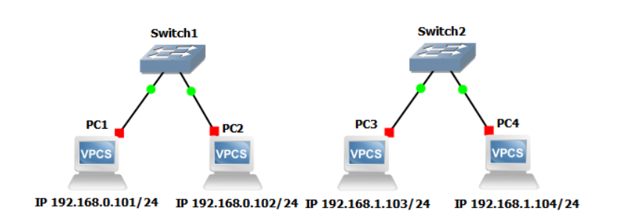
\includegraphics[width=0.8\textwidth]{images/fig1_p1a_dos_lans_sin_router.png}
    \caption{Topología inicial en GNS3.}
\end{figure}


\subsection*{1.b\quad Añadir un router (6 Puntos)}

Realice este ejercicio luego de apagar los VPCs. Para esta pregunta, se debe incorporar el router Cisco C3725 señalado en el Material de Ayuda de la tarea para obtener la topología presentada en la Figura 2.
\begin{figure}[H]
    \centering
    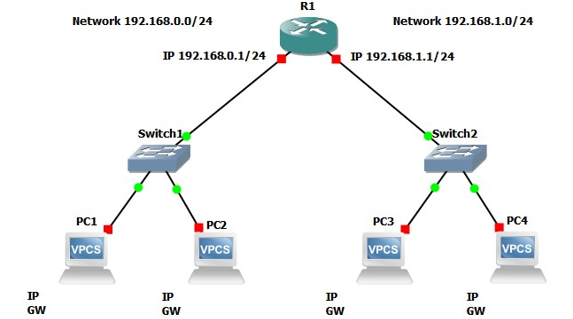
\includegraphics[width=0.8\textwidth]{images/fig2_p1b_lans_con_router_dhcp.png}
    \caption{Topología con LANs comunicadas por router en GNS3.}
\end{figure}


Para ello, haga correr la simulación y realice lo siguiente en la consola de comandos del router:

\begin{enumerate}[label=\roman*)]
    \item Asigne la IP address y máscara de red \texttt{192.168.0.1 255.255.255.0} a la interfaz fa0/0 del router.
    \item Asigne la IP address y máscara de red \texttt{192.168.1.1 255.255.255.0} a la interfaz fa0/1 del router.
    \item Investigue cómo configurar un servicio DHCP [2] e impleméntelo para cada subred, señalando \texttt{network}, \texttt{default-router} y \texttt{dns-server}. Se recomienda, y es común, configurar el router con la primera dirección IP ``asignable'' de la subred.
\end{enumerate}

Guarde la configuración del router con el comando \texttt{copy running-config startup-config}.

Para tener una referencia de este procedimiento, puede consultar en YouTube, por ejemplo \href{https://www.youtube.com/watch?v=yqjJZQjMNZc}{``DHCP Router Cisco - GNS3''}.

\textbf{En su entrega incluya la captura de la consola de comandos ejecutados en el router.}

\subsection*{1.c\quad Asignación de direcciones IP por DHCP (5 Puntos)}

Con la topología obtenida de la Figura 2, ejecute el comando necesario para la asignación de direcciones IP por DHCP para los terminales VPCs por medio de la consola de comandos para cada VPC por separado.

Ejecute el comando \texttt{save pc\_i.vpc} con $i \in \{1,2,3,4\}$ para guardar la configuración. Así se conservan los datos configurados. Para cargarlos al volver a correr un VPC, debe ejecutar el comando \texttt{load pc\_i.vpc} con $i \in \{1,2,3,4\}$. \textbf{Muestre la consola de comandos de uno de los VPCs} en su informe con las instrucciones y resultados. Actualice los cuadros de texto del diagrama de la pregunta previa con las direcciones IP y de gateways obtenidas e incluya una captura de su topología completa. Adjunte su proyecto (archivo exportado de su proyecto) en la entrega de su tarea.

\subsection*{1.d\quad Pruebas de conectividad (4 Puntos)}

Para esta pregunta, se debe corroborar la correcta implementación de las LANs. Utilizando el comando \texttt{ping} entre PC2 y cada uno de los otros tres terminales VPCs, \textbf{muestre sus resultados}.

% ==================== PREGUNTA 2 ====================
\section{Simulación de enlaces ideales y reales (25 Puntos)}

Configure una red como se muestra en la Figura 3. Ésta incluye una \textbf{máquina virtual Alpine Linux} (\href{https://profesores.elo.utfsm.cl/~agv/elo323.ipd438/2s26/Assignment/alpine-elo323-entrega.qcow2.gz}{``alpine-elo323.qcow2''}) accesible desde el Material de Ayuda \textbf{(contraseña de la máquina: \texttt{elo323})}. Para ello, debe implementar esta configuración en GNS3, incluyendo las direcciones IP señaladas para cada terminal y las características de los enlaces. Es importante considerar que uno de los enlaces de la red será configurado para producir pérdidas, limitar tasa de transferencia y definir su retardo, lo cual es emulado por la componente NETem:

\newpage
\begin{center}
\begin{tabular}{|l|c|}
    \hline
    \textbf{Bandwidth} & \textit{5 Mbps} \\ \hline
    \textbf{Delay}     & \textit{300 ms} \\ \hline
    \textbf{Loss}      & \textit{12\%} \\ \hline
\end{tabular}\\[0.2cm]
\textit{Tabla 1: Configuración de NETem}
\end{center}

Una vez iniciada la emulación del enlace con NETem, configure sus parámetros según la Tabla 1. Consulte el \textbf{Material de Ayuda} (sección \textit{NETem}) para su configuración.
\begin{figure}[H]
    \centering
    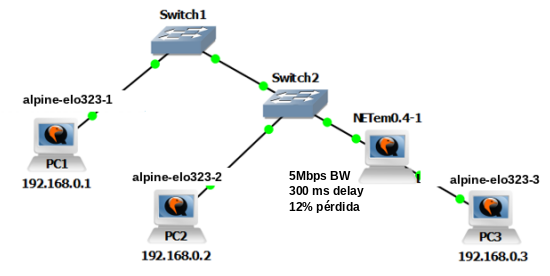
\includegraphics[width=0.8\textwidth]{images/fig3_p2_enlace_netem_alpine.png}
    \caption{Topología de red en GNS3 con enlace con pérdidas.}
\end{figure}


\subsection*{2.a\quad Pruebas de conectividad (5 Puntos)}

Utilizando el comando \texttt{ping} desde PC2, pruebe y demuestre la conectividad hacia cada uno de los terminales. Además, verifique si se cumple el retardo establecido para el enlace con limitaciones. \textbf{Muestre los resultados obtenidos}.

\subsection*{2.b\quad Intervalos de confianza (10 Puntos)}

Para este ítem, usted estimará el porcentaje de pérdida de paquetes del enlace y lo comparará con el valor configurado. Ejecute suficientes pruebas con el comando \texttt{ping} entre PC2 y PC3 y determine el porcentaje de pérdidas real del enlace con un intervalo de confianza $\pm$5\% y nivel de confianza del 95\%. \textbf{Muestre los datos y procedimiento usado para llegar a su resultado}. Para esto, puede revisar el apunte sobre \href{https://profesores.elo.utfsm.cl/~agv/elo323.ipd438/2s26/Assignment/onLinkLossEstimation_2026.pdf}{\textit{estimación de la media o promedio}}. Como sugerencia, revise las opciones \texttt{-i} y \texttt{-c} del comando \texttt{ping} al hacer las pruebas. ¿La tasa de pérdidas arrojada por ping resultó ser mayor, menor o igual a la indicada en la configuración del enlace? \textbf{Comente sus resultados}.

\subsection*{2.c\quad Mediciones de throughput (10 Puntos)}

En este ítem, usted obtendrá un valor real de throughput por medio del comando \texttt{iperf} disponible en la máquina virtual Alpine. Utilizando PC1 como servidor, PC2 y PC3 como clientes, realice la medición de tasa de transferencia con el comando \texttt{iperf}. Muestre los resultados obtenidos. En particular, para PC3 responda: ¿La tasa de transferencia medida resultó ser mayor, menor o igual a la indicada en la configuración del enlace? \textbf{Explique sus resultados}. Consulte el \textbf{Material de Ayuda} (sección \textit{iperf}).

% ==================== PREGUNTA 3 ====================
\section{RTP (25 Puntos)}

En esta actividad usted procederá a realizar transmisión de video. Usando el programa VLC, usted realizará transmisiones del tipo broadcast y unicast. Además, se visualizará el efecto de las pérdidas de paquetes en este tipo de transmisiones. Por último, para comprender el protocolo RTP, usted analizará el propósito de un par de campos de su encabezado.

\begin{nota}
En la máquina Alpine, VLC se ejecuta en modo consola con el comando \texttt{cvlc} y bajo el usuario \texttt{elo323} (no como \texttt{root}). Consulte el \textbf{Material de Ayuda} (sección \textit{Streaming con VLC}) para los comandos exactos de transmisión y recepción.
\end{nota}

\subsection*{3.a\quad Broadcast de Video (8 Puntos)}

Implemente la simulación de la Figura 4 y proceda a realizar una transmisión broadcast desde el terminal \textit{ELO323-IPD438-1} utilizando \texttt{vlc} y el archivo \texttt{sample.mp4} encontrado en la carpeta \texttt{Videos} de la máquina virtual. Inicie una captura con Wireshark en cada uno de los enlaces que van desde el switch a un terminal. ¿En cuáles de ellos circulan paquetes con el video? En los enlaces donde circulan paquetes, ¿cuál es la IP origen y la IP destino? ¿Cuál es el puerto origen y puerto destino? ¿Cuál es la MAC origen y destino? \textbf{Comente al respecto}.

\begin{figure}[H]
    \centering
    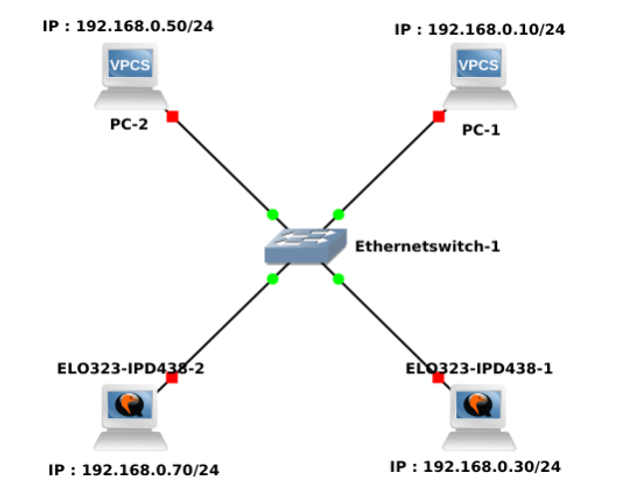
\includegraphics[width=0.5\textwidth]{images/fig4_p3a_broadcast_video_switch.png}
    \caption{Red a implementar en GNS3 para broadcast de video.}
\end{figure}


\subsection*{3.b\quad Número de Sincronización de fuente (5 Puntos)}

Para alguno de los paquetes capturados en 3.a, obtenga el número de sincronización de fuente (SSRC). Si realiza una transmisión broadcast con la máquina \textit{ELO323-IPD438-2}, ¿se sigue utilizando el mismo valor de SSRC? \textbf{Comente brevemente y respalde con capturas de paquete}.

\subsection*{3.c\quad Latencia en Transmisión de Video vía Unicast (7 Puntos)}

Implemente la red de la Figura 5, realice una transmisión unicast del video utilizado anteriormente, desde la máquina virtual Alpine y con destino a la IP de su computador personal. Aumente el retardo (\textit{delay}) paulatinamente y verifique sus efectos en la reproducción del video. ¿Existen problemas con la calidad del video? Ahora, repita las pruebas, pero configurando el parámetro \textit{jitter} igual a la mitad del \textit{delay} seleccionado. ¿Cómo afecta esto a la calidad del video? \textbf{Entregue imágenes} con los valores configurados en NETem y alguna imagen del video resultante. \textbf{Comente al respecto}.

\begin{nota}
Para que la máquina Alpine dentro de GNS3 pueda enviar el video a su computador personal, se utiliza el componente \textit{Cloud} enlazado a la interfaz de red del host. Consulte el \textbf{Material de Ayuda} (sección \textit{Componentes -- Nube}) para la configuración, incluyendo la necesidad de desactivar el firewall del host.
\end{nota}
\begin{figure}[H]
    \centering
    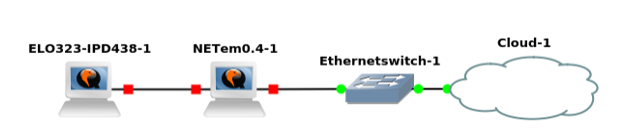
\includegraphics[width=0.8\textwidth]{images/fig5_p3c_unicast_netem_cloud.png}
    \caption{Red a implementar en GNS3 con salida a Internet.}
\end{figure}


\subsection*{3.d\quad Bandwidth en Transmisión de Video vía Unicast (5 Puntos)}

Utilizando la configuración de GNS3 del ítem anterior con los parámetros de \textit{delay} y \textit{jitter} en cero, proceda a disminuir paulatinamente la tasa de transmisión del enlace, verificando en cada prueba el estado de la recepción del video. Realice esto hasta llegar a 10 kbps.

\begin{itemize}
    \item ¿Qué fenómenos puede visualizar en la reproducción del video?
    \item ¿Ocupa VLC algún mecanismo de adaptación para sobreponerse a los cambios de tasa de transmisión en la red? Si es así, comente su observación.
\end{itemize}

% ==================== PREGUNTA 4 ====================
\section{Transmisión de llamadas VoIP (30 Puntos)}

En esta actividad se implementará un servicio de telefonía IP (VoIP) utilizando el router Cisco 3725 como servidor SIP (mediante Call Manager Express, CME) y el softphone de línea de comandos \texttt{pjsua}, disponible en la máquina Alpine. Se analizará la señalización SIP, el flujo RTP y el efecto de la degradación de red sobre la calidad de la voz.

\begin{nota}
El softphone utilizado es \texttt{pjsua} (cliente SIP por línea de comandos, parte de PJSIP). Esto permite un entorno autocontenido dentro de GNS3, liviano y representativo de servidores reales. Consulte el \textbf{Material de Ayuda} (sección \textit{Telefonía VoIP con SIP}) para la configuración del servidor SIP en el router y el uso de \texttt{pjsua}.
\end{nota}

\subsection*{4.a\quad Generación de llamada VoIP (15 Puntos)}

Implemente el esquema de red de la Figura 6, donde se establece una comunicación VoIP entre dos softphones \texttt{pjsua} conectados a través de un router Cisco 3725 configurado como servidor SIP. Los softphones se ejecutan en las máquinas Alpine. Se debe configurar el servidor SIP en el router, registrar los usuarios SIP correspondientes y configurar cada cliente \texttt{pjsua} con los parámetros asignados en el router. Una vez establecida la comunicación entre ambas máquinas, capture los paquetes de registro SIP (mensajes \texttt{REGISTER}), los paquetes de señalización de la llamada (\texttt{INVITE}, \texttt{200 OK}, \texttt{ACK}, \texttt{BYE}), así como los paquetes RTP generados por la llamada. Verifique la secuencia de mensajes de señalización, la periodicidad de los paquetes RTP y el códec de audio utilizado. Consulte el \textit{Material de Ayuda} para esta pregunta.
\begin{figure}[H]
    \centering
    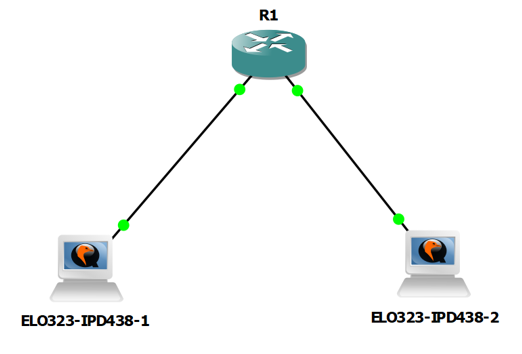
\includegraphics[width=0.6\textwidth]{images/fig6_p4a_voip_sip_router.png}
    \caption{Red a implementar en GNS3 para comunicación VoIP.}
\end{figure}


\subsection*{4.b\quad Calidad de llamada VoIP (15 Puntos)}

Implemente el esquema de red de la Figura 7. Se busca evaluar el efecto de la degradación de red sobre la calidad de una llamada VoIP. Para ello, la comunicación se establece entre \textbf{dos softphones \texttt{pjsua} ejecutándose en dos máquinas Alpine independientes}, interconectadas a través del router Cisco 3725 (servidor SIP) y con un componente \textbf{NETem intercalado en uno de los enlaces} para degradar la comunicación.

Una máquina reproduce un archivo de audio (\texttt{test\_audio.wav}, incluido en la imagen de la máquina virtual Alpine) mediante la opción \texttt{--play-file} de \texttt{pjsua}, mientras que la otra máquina graba el audio recibido mediante la opción \texttt{--rec-file}. Luego, utilizando NETem, disminuya progresivamente la tasa de transmisión y luego incremente la tasa de pérdida de paquetes del enlace. Durante cada prueba, grabe el audio recibido y analice los efectos percibidos en la calidad de la voz.

\textbf{Indique la tasa de pérdida y limitación de ancho de banda a partir de la cual el cambio en la calidad de audio comienza a ser perceptible, y aquella en la que el grupo declare la comunicación como indistinguible.} Incluya en la entrega al menos dos grabaciones de audio obtenidas desde el dispositivo receptor: una correspondiente a una condición en la que la comunicación resulte claramente comprensible y otra en la que se evidencie una degradación notable en la calidad de la voz.

\begin{nota}
Las grabaciones \texttt{.wav} obtenidas dentro de la máquina Alpine se descargan al computador personal para su análisis. Consulte el \textbf{Material de Ayuda} (sección \textit{Telefonía VoIP con SIP} y \textit{QEMU -- Montar imágenes}) para el procedimiento de extracción de los archivos.
\end{nota}
\begin{figure}[H]
    \centering
    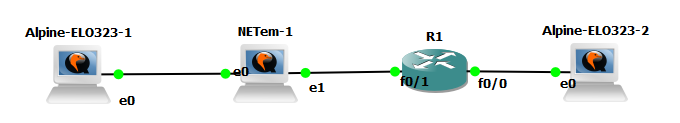
\includegraphics[width=0.8\textwidth]{images/fig7_p4b_voip_netem_calidad.png}
    \caption{Red a implementar en GNS3 para evaluación de calidad VoIP.}
\end{figure}


% ==================== REFERENCIAS ====================
\section*{Referencias}
\addcontentsline{toc}{section}{Referencias}

\begin{enumerate}[label={[\arabic*]}]
    \item \href{https://www.gns3.com/}{https://www.gns3.com/}
    \item \href{https://jmcristobal.com/es/2021/10/22/configure-dhcp-in-router-cisco/}{Configuración de DHCP en router Cisco}
    \item \href{https://docs.pjsip.org/en/latest/pjsua/pjsua.html}{PJSUA -- Command Line SIP User Agent (PJSIP)}
\end{enumerate}

\end{document}
